\begin{figure}
	
  \setlength{\unitlength}{\textwidth}

        \begin{picture}(1,0.82)(0,0.4)

      % % % Parkinson Data 

      \put(0.05,0.39){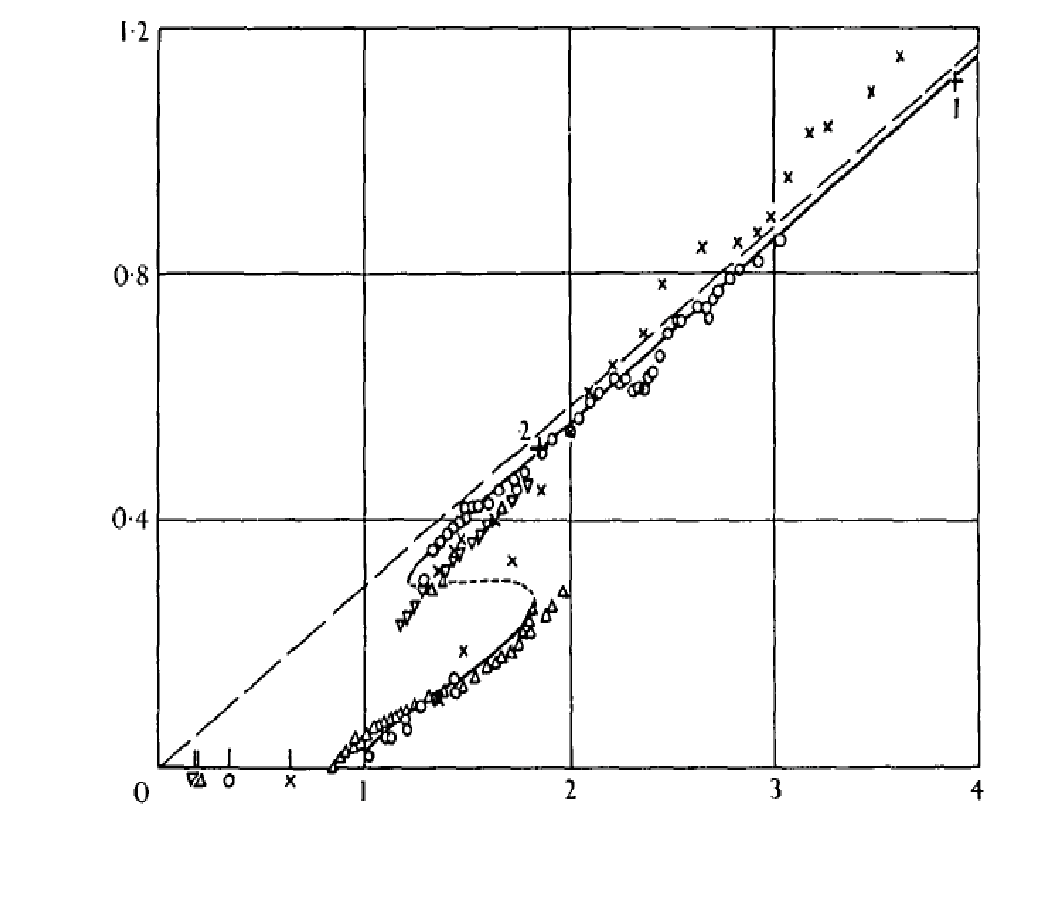
\includegraphics[width=0.9\unitlength]{./chapter-literature-revirw/fnp/parkinson_data.eps}}
      
%       \put(0.07,0.95){$\displaystyle\frac{V}{D}$}
%       \put(0.07,1.3){$\displaystyle\frac{A}{D}$}
       \put(0.05,0.8){\Large$\frac{nA}{2\beta}\bar{Y}_s$}
       \put(0.52,0.42){\Large$\frac{nA}{2\beta}U$}
       \
%\put(0.189,1.415){\small(a)}
%\put(0.189,1.07){\small(b)}
%\put(0.189,0.73){\small(c)}

%  


    \end{picture}

  \caption{``Collapsed amplitude-velocity characteristic. Theory: \solidrule \ stable limit cycle, \dashedrule unstable limit cycle. Experiment $\times \ \beta = .00107$, $\circ \ \beta =.00196$,\ $\vartriangle \beta=.00364$,$\triangledown \ \beta = .00372$,\ $+1 \ \beta=.0012$,\ $+2 \ \beta=.0032$ Reynolds numbers $4,000-20,000$ ". Figure extracted from \cite{Parkinson1964}. $\frac{nA}{2\beta}\bar{Y}_s$ is the dimensionless displacement amplitude parameter and $\frac{nA}{2\beta}U$ is the reduced velocity.}
    \label{fig:parkinson_paper_data}
\end{figure}

 %vspace{10cm}
